% !TEX program = xelatex
% !TEX encoding = UTF-8 Unicode
% گزارش یکپارچه — پروژه سوم درس نرم‌افزار ریاضی

\documentclass[a4paper,12pt,oneside]{report}

\usepackage{amsmath,amssymb}
\usepackage[table]{xcolor}
\usepackage{graphicx}
\usepackage{float}
\usepackage{subcaption}
\usepackage{booktabs}
\usepackage{listings}
\usepackage{titlesec}
\usepackage{caption}
\usepackage{fancyhdr}
\usepackage{enumitem}
\usepackage[bottom]{footmisc}
\usepackage[breaklinks=true,hidelinks]{hyperref}
\usepackage[top=2.8cm,right=2.8cm,bottom=2.8cm,left=2.5cm]{geometry}

\makeatletter
\g@addto@macro\@floatboxreset\centering
\makeatother

\usepackage{xepersian}
\settextfont[Scale=1.13,Ligatures=TeX]{IRNazanin}
\setdigitfont[Scale=1.13]{IRNazanin}
\setlatintextfont[Scale=1.06,Ligatures=TeX]{Times New Roman}

% ── style.tex ──
% ── Colors & helpers ──
\definecolor{autblue}{RGB}{0,72,140}
\definecolor{textgray}{RGB}{80,80,90}
\definecolor{codebg}{RGB}{248,250,252}
\definecolor{codeframe}{RGB}{210,218,228}
\definecolor{keywordcolor}{RGB}{0,80,160}

\newcommand{\githublink}{%
  \begin{center}
  \vspace{0.3em}
  \href{https://github.com/melikazre/numerical-analysis}{\lr{github.com/melikazre/numerical-analysis}}
  \vspace{0.3em}
  \end{center}
}

\captionsetup{
  font=small,
  labelfont={bf,color=autblue},
  skip=10pt,
  justification=centering,
}

% ── Persian listing captions (RTL, no English "Listing") ──
\newcommand{\listingtitle}[1]{%
  \refstepcounter{lstlisting}%
  \par\vspace{0.5em}%
  \begin{center}%
  {\small\bfseries\color{autblue}\begin{RTL}#1 \textendash\ برنامه~\thelstlisting\end{RTL}}%
  \end{center}%
  \vspace{0.3em}%
}

\AtBeginDocument{%
  \renewcommand{\lstlistingname}{برنامه}%
}

\lstdefinestyle{pythonstyle}{
  language=Python,
  basicstyle=\ttfamily\scriptsize,
  keywordstyle=\color{keywordcolor}\bfseries,
  commentstyle=\color{textgray}\itshape,
  stringstyle=\color{teal},
  numbers=left,
  numberstyle=\tiny\color{textgray},
  stepnumber=1,
  numbersep=6pt,
  backgroundcolor=\color{codebg},
  frame=single,
  rulecolor=\color{codeframe},
  breaklines=true,
  showstringspaces=false,
  tabsize=4,
  xleftmargin=10pt,
  framexleftmargin=10pt,
  aboveskip=1em,
  belowskip=1em,
}
\lstdefinestyle{outputstyle}{
  basicstyle=\ttfamily\scriptsize,
  backgroundcolor=\color{codebg},
  frame=single,
  rulecolor=\color{codeframe},
  breaklines=true,
  showstringspaces=false,
  tabsize=4,
  xleftmargin=10pt,
  framexleftmargin=10pt,
  aboveskip=1em,
  belowskip=1em,
  numbers=none,
}

\lstset{style=pythonstyle}


% ── فاصله خطوط و پارagraph ──
\linespread{1.6}
\setlength{\parskip}{0.65em}
\setlength{\parindent}{0pt}

% ── لیست‌ها (RTL) ──
\setlist[itemize,1]{rightmargin=0pt,leftmargin=1.6em,itemsep=0.4em,topsep=0.6em}
\setlist[enumerate,1]{rightmargin=0pt,leftmargin=1.6em,itemsep=0.4em,topsep=0.6em}

% ── عناوین + فاصله تا متن بعد ──
\titleformat{\chapter}[display]
  {\RTL\bfseries\color{autblue}}
  {\huge\chaptertitlename~\thechapter}
  {1.2ex}
  {\Huge}
  [\vspace{0.6ex}{\color{autblue}\hrule height 0.8pt}\vspace{1.4ex}]

\titlespacing*{\chapter}{0pt}{0pt}{0pt}

\titleformat{\section}
  {\RTL\Large\bfseries\color{autblue}}
  {\thesection}{0.6em}{}
  [\vspace{1.2ex}]

\titlespacing*{\section}{0pt}{1.8em}{0.8em}

\titleformat{\subsection}
  {\RTL\large\bfseries\color{textgray}}
  {\thesubsection}{0.5em}{}
  [\vspace{0.8ex}]

\titlespacing*{\subsection}{0pt}{1.4em}{0.6em}

\setlength{\headheight}{16pt}
\setlength{\floatsep}{16pt}
\setlength{\textfloatsep}{20pt}

\pagestyle{fancy}
\fancyhf{}
\fancyhead[R]{\small\thepage}
\fancyhead[L]{\small\leftmark}
\renewcommand{\headrulewidth}{0.3pt}

\graphicspath{{./}{../results/}}

% ── constants.tex ──
% these are some protocols to follow in this document...

% define gaps here...
\newcommand{\smallGap}{\\ [.2cm]}
\newcommand{\mediumGap}{\\ [.5cm]}
\newcommand{\bigGap}{\\ [1cm]}
% ── cover_info.tex ──
% define some string variables...
\newcommand{\universityTitle}{دانشگاه صنعتی امیرکبیر}
\newcommand{\universityLink}{http://aut.ac.ir}
\newcommand{\universitySubTitle}{پلی‌تکنیک تهران}
\newcommand{\departement}{دانشکده علوم ریاضی}
\newcommand{\departementLink}{http://aut.ac.ir}
\newcommand{\reportType}{پروژه سوم درس نرم‌افزار ریاضی}
\newcommand{\field}{}
\newcommand{\reportTitle}{درونیابی، تحلیل زمان اجرای الگوریتم‌ها و انتگرال‌گیری عددی}
\newcommand{\reportAuthor}{ملیکا زارع}
\newcommand{\reportAuthorLink}{https://github.com/melikazre/numerical-analysis}
\newcommand{\instructor}{استاد حسینقلی زاده}
\newcommand{\examinerFirst}{}
\newcommand{\examinerSecond}{}
\newcommand{\reportDate}{تیر ۱۴۰۴}
% ── functions.tex ──
% here's some helper functions needed...

% check if variable defined...
\newcommand {\isDefined} [3] {
	% fist check if variable is defined...
	\ifdefined #1
		% then check if the variable is not dumping strings...
		\setbox0=\hbox{#1\unskip}\ifdim\wd0=0pt
			% variable assumed not-defined...
			#3
		\else
			% variable assumed defined...
			#2
		\fi
	\else
		% variable assumed not-defined...
		#3
	\fi
}


\renewcommand{\thesection}{\arabic{section}.\arabic{chapter}}
\renewcommand{\thesubsection}{\arabic{subsection}.\arabic{section}.\arabic{chapter}}
\renewcommand{\theequation}{\arabic{equation}.\arabic{chapter}}
\renewcommand{\thefigure}{\arabic{figure}.\arabic{chapter}}
\renewcommand{\thetable}{\arabic{table}.\arabic{chapter}}

\begin{document}

% ── cover ──
\thispagestyle{empty}
\enlargethispage{1cm}

\begin{center}
  \vspace*{0.15cm}
  
\includegraphics[width=0.17\textwidth]{logo.png}

  \vspace{0.55cm}
  {\color{autblue}\rule{0.48\textwidth}{1pt}}

  \vspace{0.45cm}
  {\LARGE\bfseries\color{autblue}\universityTitle}\\[0.25cm]
  {\large (\universitySubTitle)}

  \vspace{0.35cm}
  {\large\departement}

  \vspace{0.9cm}
  {\normalsize\color{textgray}\reportType}

  \vspace{0.55cm}
  {\normalsize عنوان}\\[0.25cm]
  {\Large\bfseries\reportTitle}

  \vspace{0.9cm}
  {\normalsize نگارش}\\[0.2cm]
  {\large\bfseries\reportAuthor}

  \vspace{0.55cm}
  {\normalsize استاد درس}\\[0.2cm]
  {\large\instructor}

  \vspace{0.7cm}
  {\color{autblue}\rule{0.28\textwidth}{0.6pt}}\\[0.35cm]
  {\normalsize\reportDate}
\end{center}

\clearpage

\pagenumbering{arabic}

% ── 1-introduction ──
\chapter{مقدمه}
\label{ch:introduction}

\noindent
در این پروژه سه مسئله‌ی اصلی با \lr{Python} پیاده‌سازی شده و نتایج هر بخش به‌همراه کد، خروجی و نمودار گزارش می‌شود.

\vspace{0.5em}
\noindent\textbf{خلاصه‌ی کارهای انجام‌شده:}
\begin{enumerate}
  \item \textbf{بخش ۱:} درونیابی نقاط \lr{(1,1)} تا \lr{(6,2)} با لاگرانژ و اسپلاین و استخراج ضابطه‌ی دقیق
  \item \textbf{بخش ۲:} خواندن خودکار \lr{Excel}، رسم نمودارهای میله‌ای/خطی/جعبه‌ای، افزودن \lr{700KB} و محاسبه‌ی میانگین \lr{Alg.2}
  \item \textbf{بخش ۳:} انتگرال‌گیری $f(x)=e^{x^2}$ روی $(0,1)$ با ذوزنقه‌ای، سیمسون و گاوس
  \item \textbf{بخش ۵:} قرار دادن کدها در \lr{Repository} عمومی \lr{GitHub}
\end{enumerate}

\section{فایل‌های \lr{Python}}
\begin{itemize}
  \item \lr{lagrange\_and\_spline.py} \hfill بخش ۱
  \item \lr{runtime\_from\_excel.py} \hfill بخش ۲
  \item \lr{integrate\_exp\_square.py} \hfill بخش ۳
  \item \lr{main.py} \hfill اجرای یک‌جای همه‌ی بخش‌ها
\end{itemize}

\section{\lr{Repository}}
\githublink

% ── 2-related_works ──
\chapter{بخش ۱: درونیابی لاگرانژ و اسپلاین}
\label{ch:interpolation}

\section{شرح مسئله}
طبق بخش ۱ پروژه، نقاط زیر در نظر گرفته شده‌اند:
\[
(1,1),\;(2,3),\;(3,5),\;(4,8),\;(5,5),\;(6,2)
\]
باید این داده‌ها با \textbf{درونیابی لاگرانژ} و \textbf{اسپلاین} درون‌یابی شوند و \textbf{ضابطه‌ی دقیق} هر روش به‌دست آید.

\section{روش پیاده‌سازی}
در لاگرانژ، چندجمله‌ای درجه‌ی $5$ ساخته می‌شود:
\begin{equation}
L(x)=\sum_{i=0}^{n-1} y_i\,\ell_i(x),
\qquad
\ell_i(x)=\prod_{\substack{j=0\\ j\neq i}}^{n-1}\frac{x-x_j}{x_i-x_j}
\end{equation}

در اسپلاین مکعبی طبیعی، در هر بازه‌ی $[x_i,x_{i+1}]$:
\begin{equation}
S_i(x)=a_i+b_i(x-x_i)+c_i(x-x_i)^2+d_i(x-x_i)^3
\end{equation}

\section{کد \lr{Python}}
\listingtitle{\lr{lagrange\_and\_spline.py}}
\begin{LTR}
\lstinputlisting[style=pythonstyle]{../lagrange_and_spline.py}
\end{LTR}

\section{خروجی برنامه}
\listingtitle{خروجی اجرای بخش ۱}
\begin{LTR}
\begin{lstlisting}[style=outputstyle]
Part 1 - Lagrange and spline interpolation

Data points:
  (1, 1)  (2, 3)  (3, 5)  (4, 8)  (5, 5)  (6, 2)

Lagrange formula:
  L(x) = 0.175*x**5 - 2.95833333333333*x**4
       + 18.375*x**3 - 52.0416666666667*x**2
       + 68.45*x - 31.0

Spline pieces:
  interval [1, 2]: S1(x) = -0.1866 + 0.0000(x-1.0)
       + 2.1866(x-1.0)^2 + 1.0000(x-1.0)^3
  interval [2, 3]: S2(x) = 0.9330 + -0.5598(x-2.0)
       + 1.6268(x-2.0)^2 + 3.0000(x-2.0)^3
  interval [3, 4]: S3(x) = -2.5455 + 2.2392(x-3.0)
       + 3.3062(x-3.0)^2 + 5.0000(x-3.0)^3
  interval [4, 5]: S4(x) = 2.2488 + -5.3971(x-4.0)
       + 0.1483(x-4.0)^2 + 8.0000(x-4.0)^3
  interval [5, 6]: S5(x) = -0.4498 + 1.3493(x-5.0)
       + -3.8995(x-5.0)^2 + 5.0000(x-5.0)^3
\end{lstlisting}
\end{LTR}

\section{ضابطه‌ی دقیق لاگرانژ}
\[
\boxed{L(x)=0.175x^5-2.958\overline{3}x^4+18.375x^3-52.041\overline{6}x^2+68.45x-31}
\]

\section{نمودار}
\begin{figure}[H]
\centering
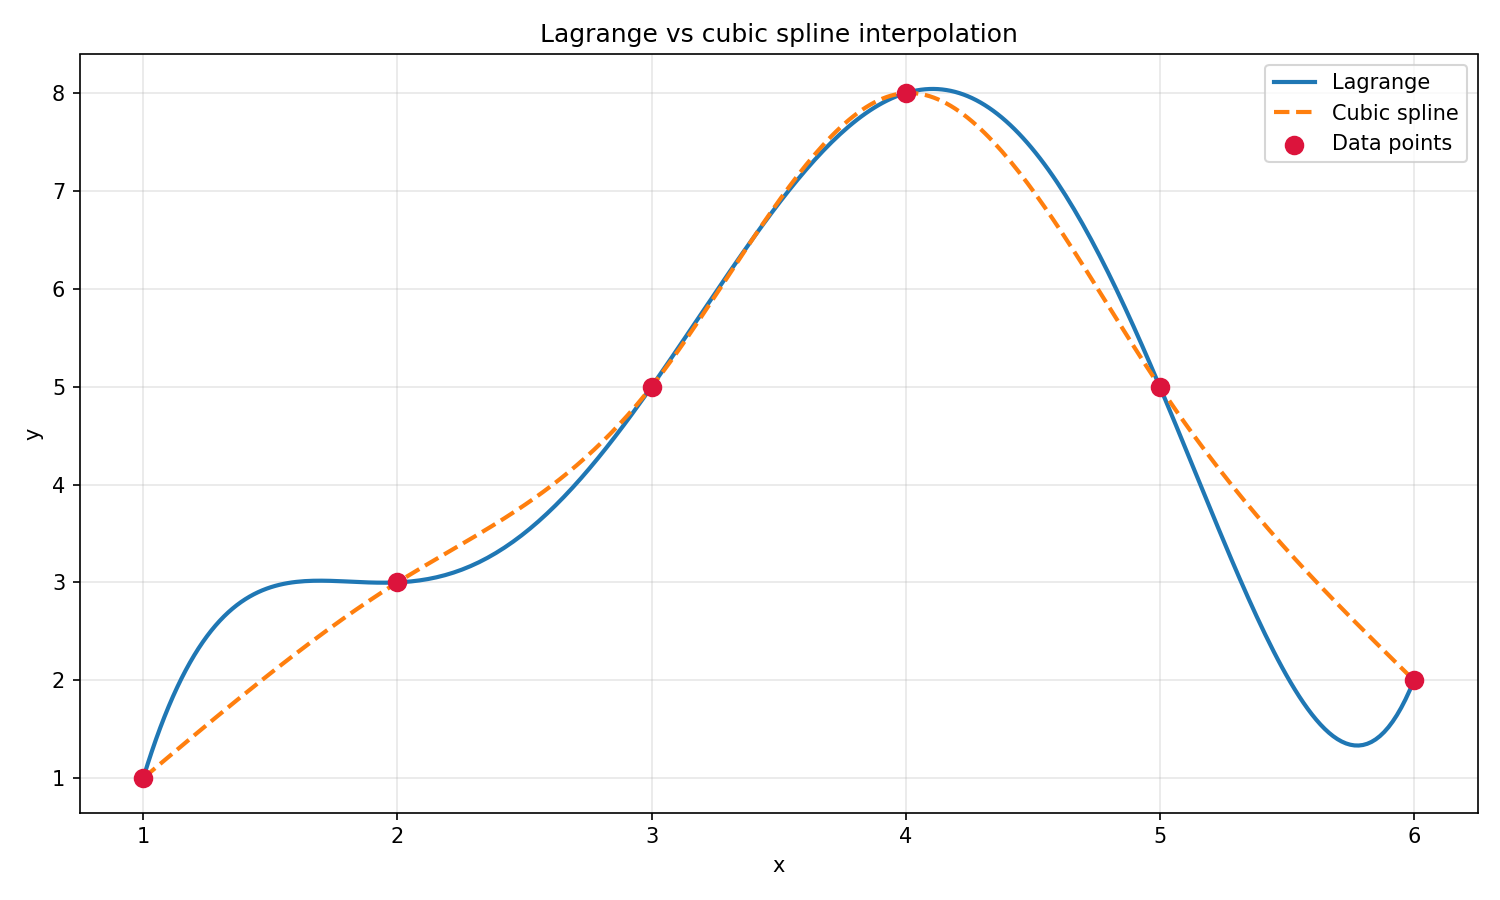
\includegraphics[width=0.82\textwidth]{interpolation_plot.png}
\caption{مقایسه‌ی منحنی‌های لاگرانژ و اسپلاین}
\label{fig:interp}
\end{figure}

\section{تحلیل}
\begin{itemize}
  \item هر دو روش از تمام شش نقطه می‌گذرند.
  \item \textbf{لاگرانژ:} در بازه‌ی $[4,6]$ نوسان شدید دارد (\lr{Runge phenomenon}).
  \item \textbf{اسپلاین:} منحنی هموارتر و پایدارتر است.
  \item برای این داده‌ها، اسپلاین برای نمایش و تفسیر مناسب‌تر است.
\end{itemize}

% ── 3-proposed_method ──
\chapter{بخش ۲: تحلیل زمان اجرا از \lr{Excel}}
\label{ch:runtime}

\section{شرح مسئله}
فایل \lr{runtime\_data.xlsx} زمان اجرای \lr{Alg.1}، \lr{Alg.2} و \lr{Alg.3} را برای اندازه‌های \lr{100KB} تا \lr{600KB} (و سطر \lr{700KB}) ذخیره کرده است.

\section{کد \lr{Python}}
\listingtitle{\lr{runtime\_from\_excel.py}}
\begin{LTR}
\lstinputlisting[style=pythonstyle]{../runtime_from_excel.py}
\end{LTR}

\section{بخش ۲-الف: خواندن \lr{Excel} و رسم نمودار}
کد با \lr{pandas.read\_excel} تمام سطرها و ستون‌ها را \textbf{بدون ورود دستی} می‌خواند و سه نمودار میله‌ای، خطی و جعبه‌ای رسم می‌کند.

\begin{table}[H]
\centering
\renewcommand{\arraystretch}{1.35}
\caption{داده‌های خوانده‌شده از \lr{Excel}}
\label{tab:runtime}
\begin{latin}
\begin{tabular}{lrrr}
\toprule
Data size & Alg.1 & Alg.2 & Alg.3 \\
\midrule
100KB & 50  & 200 & 100 \\
200KB & 55  & 220 & 200 \\
300KB & 60  & 240 & 300 \\
400KB & 65  & 260 & 400 \\
500KB & 70  & 280 & 500 \\
600KB & 75  & 300 & 600 \\
700KB & 80  & 320 & 700 \\
\bottomrule
\end{tabular}
\end{latin}
\end{table}

\begin{figure}[H]
\centering
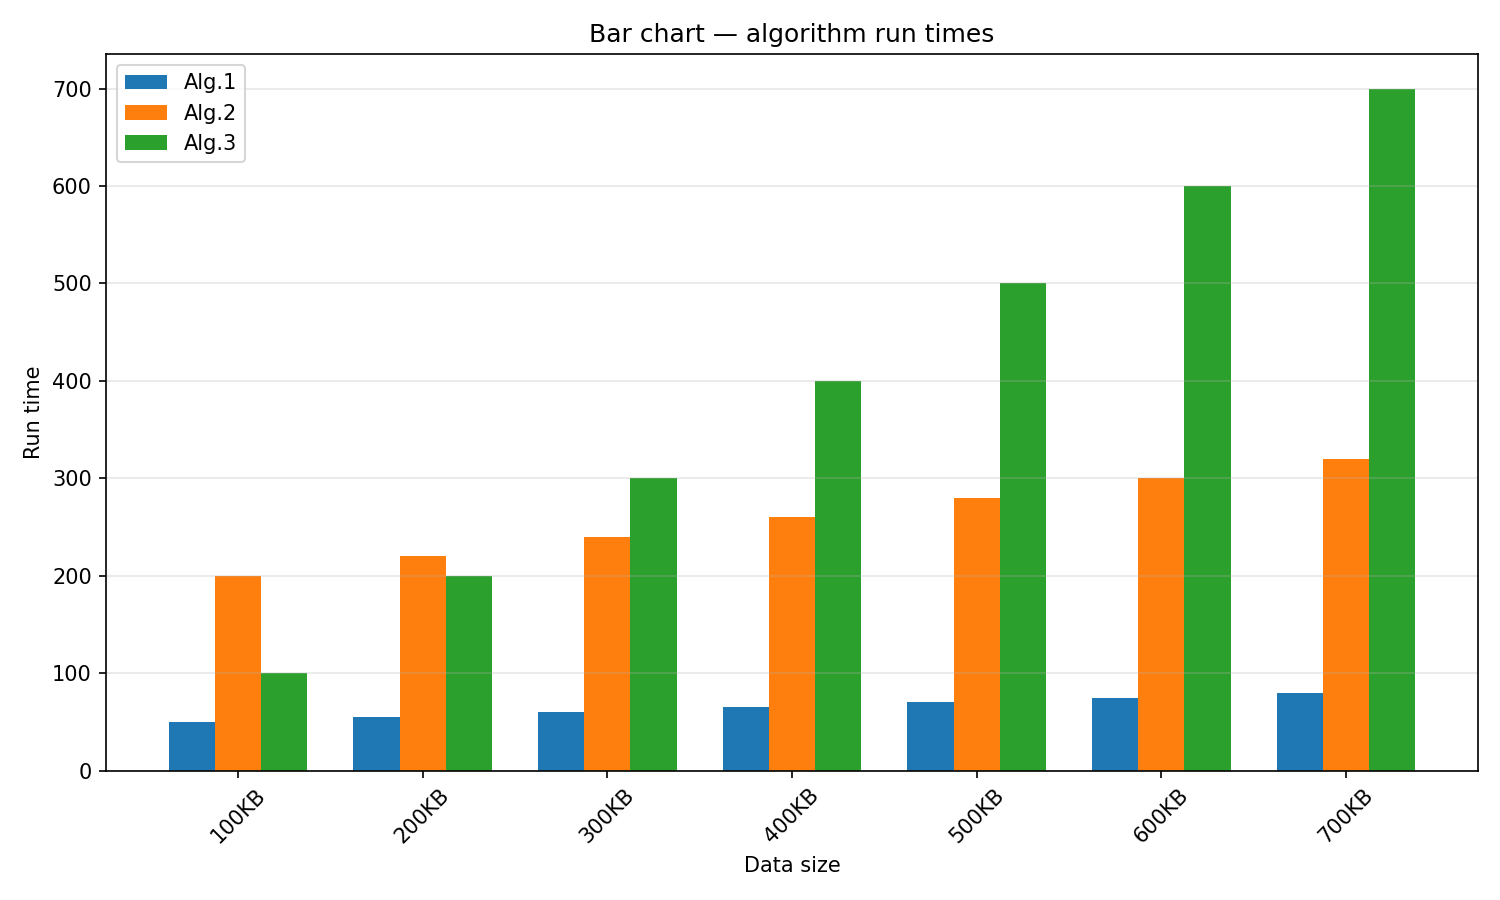
\includegraphics[width=0.85\textwidth]{runtime_bar_chart.png}
\caption{نمودار میله‌ای (بخش ۲-الف)}
\label{fig:bar}
\end{figure}

\textbf{تحلیل نمودار میله‌ای:}
\lr{Alg.3} بیشترین زمان را دارد. \lr{Alg.1} سریع‌ترین الگوریتم است. با افزایش اندازه‌ی داده، زمان هر سه الگوریتم بیشتر می‌شود.

\begin{figure}[H]
\centering
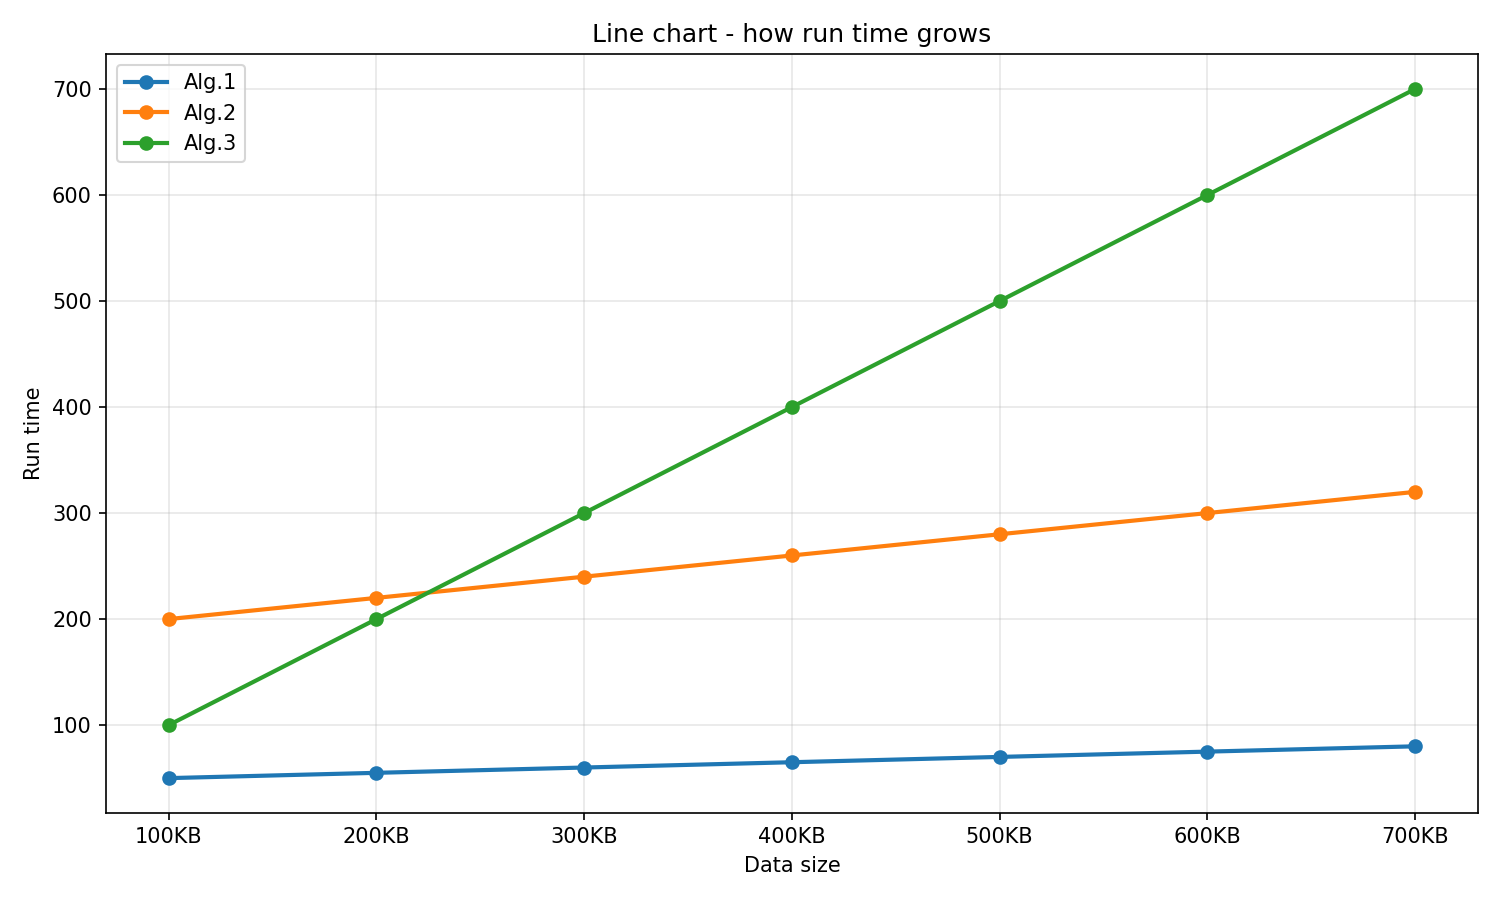
\includegraphics[width=0.85\textwidth]{runtime_line_chart.png}
\caption{نمودار خطی (بخش ۲-الف)}
\label{fig:line}
\end{figure}

\textbf{تحلیل نمودار خطی:}
\lr{Alg.3} تقریباً خط راست با شیب $1$ است (زمان $\approx$ اندازه‌ی داده). \lr{Alg.2} رشد خطی با شیب کمتر دارد. \lr{Alg.1} کندترین رشد را دارد.

\begin{figure}[H]
\centering
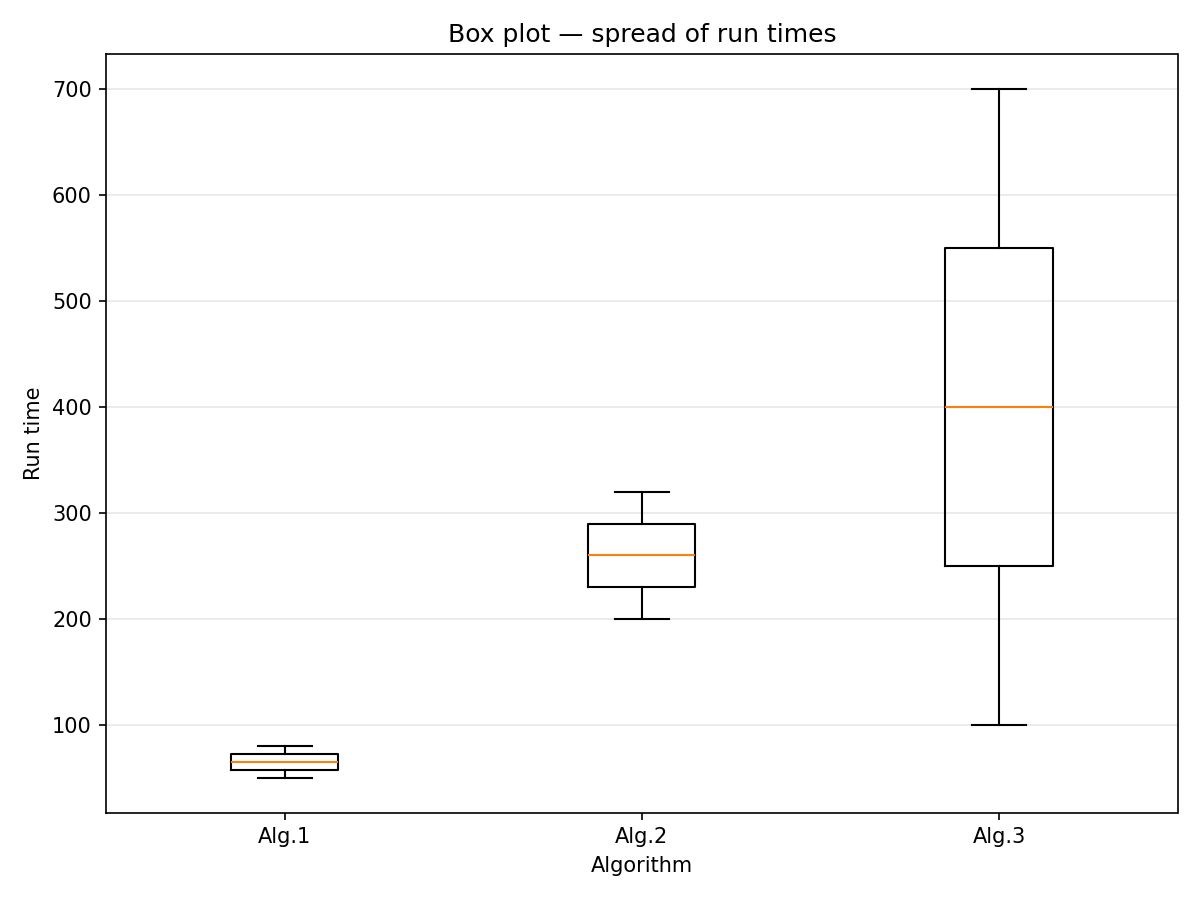
\includegraphics[width=0.72\textwidth]{runtime_box_plot.png}
\caption{نمودار جعبه‌ای (بخش ۲-الف)}
\label{fig:box}
\end{figure}

\textbf{تحلیل نمودار جعبه‌ای:}
\lr{Alg.1} کم‌ترین پراکندگی (\lr{50}--\lr{80}) را دارد. \lr{Alg.3} بیشترین دامنه (\lr{100}--\lr{700}) و حساس‌ترین الگوریتم به اندازه‌ی داده است.

\section{بخش ۲-ب: افزودن سطر \lr{700KB}}
سطر زیر به \lr{Excel} اضافه شده است:
\begin{latin}
\begin{tabular}{lrrr}
700KB & 80 & 320 & 700 \\
\end{tabular}
\end{latin}
با اجرای مجدد کد \textbf{بدون هیچ تغییری}، نمودارها به‌روز شدند و سطر \lr{700KB} در جدول و نمودارها دیده می‌شود.

\section{بخش ۲-ج: میانگین \lr{Alg.2}}
\listingtitle{خروجی میانگین \lr{Alg.2}}
\begin{LTR}
\begin{lstlisting}[style=outputstyle]
Average Alg.2 for 100-600 KB:
  values: [200, 220, 240, 260, 280, 300]
  mean:   250.00
\end{lstlisting}
\end{LTR}

\[
\bar{t}_{\mathrm{Alg.2}}=\frac{200+220+240+260+280+300}{6}=250.00
\]

میانگین زمان اجرای \lr{Alg.2} برای داده‌های \lr{100KB} تا \lr{600KB} برابر \textbf{\lr{250.00}} است.

% ── 4-evaluation ──
\chapter{بخش ۳: انتگرال‌گیری $f(x)=e^{x^2}$}
\label{ch:integration}

\section{شرح مسئله}
تابع $f(x)=e^{x^2}$ در نظر گرفته شده و مقدار انتگرال روی $(0,1)$ محاسبه می‌شود:
\[
I=\int_0^1 e^{x^2}\,dx
\]

\section{کد \lr{Python}}
\listingtitle{\lr{integrate\_exp\_square.py}}
\begin{LTR}
\lstinputlisting[style=pythonstyle]{../integrate_exp_square.py}
\end{LTR}

\section{بخش ۳-الف: ذوزنقه‌ای و سیمسون}
\begin{equation}
I\approx h\left[\frac{f(a)+f(b)}{2}+\sum_{i=1}^{n-1}f(x_i)\right]
\qquad\text{(ذوزنقه‌ای)}
\end{equation}
\begin{equation}
I\approx\frac{h}{3}\left[f(a)+f(b)+4\sum_{\mathrm{odd}} f(x_i)+2\sum_{\mathrm{even}} f(x_i)\right]
\qquad\text{(سیمسون)}
\end{equation}

\section{بخش ۳-ب: گاوس--لژاندر و مقایسه}
انتگرال با \lr{10} نقطه‌ی گاوس روی $[-1,1]$ محاسبه و به بازه‌ی $[0,1]$ نگاشت شده است. نتایج با \lr{scipy.integrate.quad} مقایسه شده‌اند.

\begin{table}[H]
\centering
\renewcommand{\arraystretch}{1.4}
\caption{مقایسه‌ی روش‌های انتگرال‌گیری (بخش ۳)}
\label{tab:integral}
\begin{latin}
\begin{tabular}{lcc}
\toprule
Method & Value & Error vs reference \\
\midrule
Trapezoidal ($n=1000$) & 1.4626521990 & $4.53\times10^{-7}$ \\
Simpson ($n=1000$)     & 1.4626517459 & $3.02\times10^{-13}$ \\
Gauss (10 points)      & 1.4626517459 & $6.66\times10^{-16}$ \\
Reference (scipy)      & 1.4626517459 & --- \\
\bottomrule
\end{tabular}
\end{latin}
\end{table}

\listingtitle{خروجی اجرای بخش ۳}
\begin{LTR}
\begin{lstlisting}[style=outputstyle]
Part 3 - integrating f(x) = e^(x^2) on (0, 1)

Trapezoidal (n=1000):  1.4626521990
Simpson (n=1000):       1.4626517459
Gauss (10 points):          1.4626517459
Reference (scipy):          1.4626517459

Error vs reference:
  trapezoidal: 4.53e-07
  simpson:     3.02e-13
  gauss:       6.66e-16
\end{lstlisting}
\end{LTR}

\section{تحلیل مقایسه‌ای}
\begin{itemize}
  \item \textbf{ذوزنقه‌ای:} ساده است اما با $n=1000$ هنوز خطای $4.53\times10^{-7}$ دارد.
  \item \textbf{سیمسون:} با همان $n=1000$ تقریباً با مرجع یکسان است (خطای $10^{-13}$).
  \item \textbf{گاوس:} تنها با \lr{10} ارزیابی تابع به دقت ماشین ($10^{-16}$) می‌رسد.
  \item \textbf{نتیجه:} برای $e^{x^2}$ روی $[0,1]$، سیمسون و گاوس از ذوزنقه‌ای دقیق‌ترند؛ گاوس بهترین نسبت دقت به هزینه را دارد.
\end{itemize}

% ── 5-conclusion ──
\chapter{نتیجه‌گیری}
\label{ch:conclusion}

در این پروژه تمام موارد خواسته‌شده پیاده‌سازی و گزارش شد:

\begin{enumerate}
  \item \textbf{بخش ۱:} ضابطه‌ی لاگرانژ و پنج قطعه‌ی اسپلاین استخراج شد. اسپلاین هموارتر از لاگرانژ بود.
  \item \textbf{بخش ۲:} \lr{Excel} خودکار خوانده شد؛ سه نمودار رسم و تحلیل شد. سطر \lr{700KB} بدون تغییر کد اضافه شد. میانگین \lr{Alg.2} برابر \lr{250.00} شد.
  \item \textbf{بخش ۳:} $I \approx 1.4626517459$ محاسبه شد. سیمسون و گاوس دقیق‌تر از ذوزنقه‌ای بودند.
  \item \textbf{بخش ۵:} کدها در \lr{Repository} عمومی \lr{GitHub} قرار گرفتند.
\end{enumerate}

\end{document}
